\chapter{Introdução e Contexto}
A memória \emph{DRAM}, do inglês \emph{Dynamic Random-access Memory}, é um tipo de memória volátil de acesso aleatório, ou seja, seus dados podem ser acessados
em tempo aproximadamente constante independentemente de sua posição na memória. Por ser estruturalmente simples (apenas um transistor e um capacitor por bit) sua densidade é muito maior do que outros tipos de memória (SRAM utiliza até 6 transistores por bit) e, apesar de necessitar que seus capacitores sejam recarregados constantemente para manter os dados, tornou-se assim a memória principal na grande maioria dos computadores.

Nos últimos 15 anos o uso de memória DRAM em sistemas de armazenamento de dados vem aumentando para atender às necessidades de aplicações web de larga escala. Isso
ocorre principalmente porque embora a capacidade de armazenamento dos discos rígidos (hard disk ou HD, em inglês) tenha aumentado exponencialmente, tanto sua latência de acesso quanto sua vazão de dados não evoluiram na mesma proporção~\ref{fig:i0}. Essa aplicações web lidam necessitam lidar com um grande volume de dados em uma intensidade que um sistema de armazenamento baseado puramente em disco ou memória flash não conseguiriam atender, o que faz com que cada vez mais dados precisem estar disponíveis em memória RAM. Como exemplo, sistemas de busca como o Google ou o Yahoo mantém toda sua estrutura de índices em DRAM.

Embora o uso massivo de memória ram venha crescendo, sua principal utilização para sistemas de armazenamento de dados é na forma de \emph{cache}. Nesse caso a aplicação tem que ficar responsável por manter o cache coerente com a base de dados, o que aumenta sua complexidade e limita o seu desempenho pela quantidade de erros de coerência do cache (\emph{cache misses}).

O projeto RAMCloud é um sistema de armazenamento que propõe manter os dados em DRAM de modo persistente e distribuido. Suas três premissas são: baixa latência, escalabilidade e durabilidade. Quando utilizado em um \emph{cluster} interligado por redes de tecnologia de ponta (por exemplo redes \emph{Infiniband}) atinge a latência de 5$\mu$s para leitura e 15$\mu$s para escrita. Esse cluster pode ser composto facilmente por 10.000 máquinas com um único sistema de endereçamento de 
dados do tipo chave-valor, o que implica em uma capacidade inicial de 1PB de DRAM. Para garantir a durabilidade e a disponibilidade os dados também são armazenados em um sistema secundário baseado em disco, de um modo que não degrade o desempenho do sistema e que permita a recuperação em caso de falha em menos de dois segundos. 

\begin{figure}[H]\centering
  \centerline{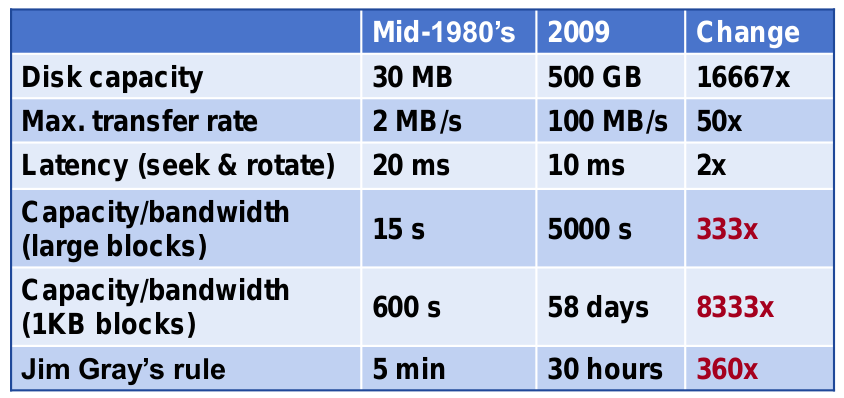
\includegraphics[width=\textwidth]{figuras/i0.png}}
  \caption{Comparação entre disco rigidos com 25 anos de diferença. Os números em vermelho indicam o quanto piorou o desempenho}\label{fig:i0}
\end{figure} 


